\chapterimage{Chapter14.jpg} % Chapter heading image

\chapter{Sludge Thickening}

			Prior to the sludge stabilization process such as anaerobic digestion, the solids content of the sludge is increased by utilizing an appropriate thickening process.\\
			Notes:\\
			1) There is an upper limit of the solids concentration that can be effectively treated as increasing the solids concentration reduces its ability to be mixed and pumped easily. Digesters can effectively treat sludges with upto about maximum 7\% - 9\% solids.\\
			2) If a 5000 mg/l (0.5\%) sludge is thickened to 5\% solids concentration - it will reduce the volume of sludge by 90\%\\

\section{Advantages of sludge thickening}\index{Advantages of sludge thickening}

		\begin{itemize}
			\item Improved digester performance due to a lower volume of sludge
			\item Capital Cost savings associated with less digester volume requirements
			\item Operational costs savings - for sludge heating and mixing
		\end{itemize}
        
\section{Sludge thickening methods}\index{Sludge thickening methods}

		\begin{enumerate}
			\item Gravity thickener - more suitable for primary sludge
			\item Dissolved air floatation thickener - more suitable for lighter, fluffier floc such as the secondary sludge.
		\end{enumerate}
\section{Gravity thickener}\index{Gravity thickener}
The gravity thickener is designed and operated similar to a circular primary and secondary clarifier.
\begin{center}
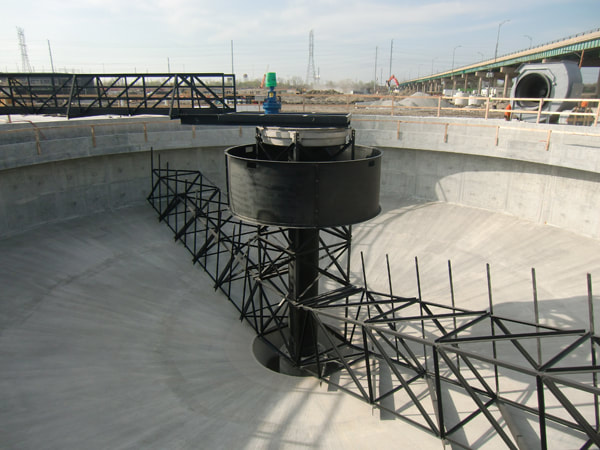
\includegraphics[scale=0.45]{GravityThickener}\\
\vspace{1cm}
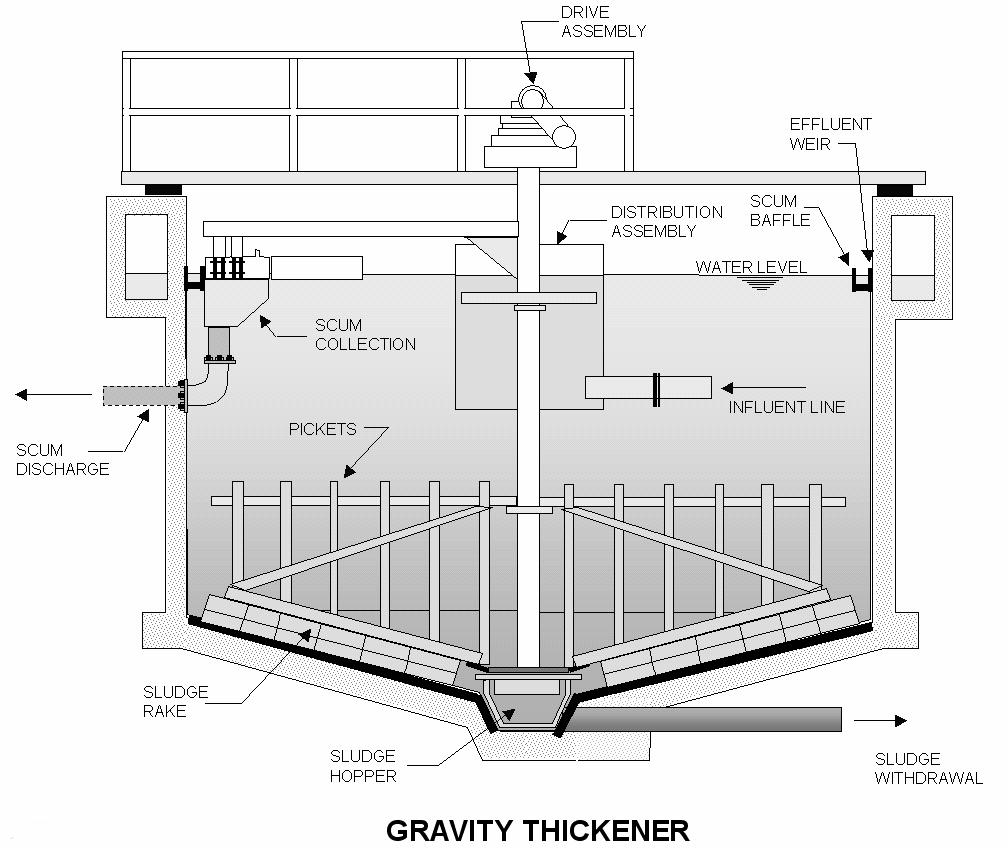
\includegraphics[scale=0.45]{ThickenerGravityThickener}
\vspace{1cm}
\end{center}
\subsection{Principles of gravity thickener operations}\index{Principles of gravity thickener operations}
   
\begin{itemize}
\item Upon entering the tank from the center, the sludge solids settle under the influence of gravity and these settled solids accumulate in the bottom of the gravity thickener as the sludge blanket.  As the sludge becomes thicker it helps squeeze out more water from the sludge increasing the sludge solids content.
\item Typical solids loading rates of a gravity thickener used for thickening primary sludge is 20-30 lbs TS/day-ft$^2$
\item A picket fence-like mechanism which is attached to the bottom sludge rake arms is primarily to release entrapped gases.  The sludge rake arms rotate at a very slow speed to ensure that it does not cause turbulenece causing the sludge to rise.  The sludge is gently raked towards a sump in the center, from where the solids are withdrawn.  The sludge rake encounter much higher torques than the typical primary clarifier rake, and is therefore designed to be more stronger and heftier. 
\item The thickened solids are drawn-off at regular intervals and the liquid fraction is decanted from the top and returned to the primary clarifier.  The typical sludge concentration factor is about 2.
\item The sludge blanket is kept about three feet.  
\item The sludge blanket depth is typically maintained so that the sludge does not turn septic and the effluent is relatively clear and free of solids.  
\item Sludge Volume ratio (SVR) provides a means of regulating the detention time of sludge within the blanket of the thickener
\item SVR is defined as the volume of the sludge blanket divided by the daily volume Of sludge pumped from the thickener. 
\item SVR is a relative measure of the average detention time of solids in the thickener and is calculated in days.
\item Typical SVRs for primary sludge range from 0.5 - 2 days.
\item Scum is removed from the top using a separate scum removal mechanism.

\item Chemical additives may be utilized to enhance settling and control odors.
\end{itemize}

\subsection{Elements of a gravity thickener}\index{Elements of a gravity thickener}

\begin{itemize}
\item center feed column and baffle\\
\item drive assembly\\
\item scum removal system\\
\item thickened sludge pump\\
\item sludge rake with pickets\\
\item effluent weir\\
\item sludge hopper and pump\\
\end{itemize}

\subsection{Gravity thickener operational parameters}\index{Gravity thickener operational parameters}

\begin{itemize}
\item type and quality of sludge\\
\item hydraulic or surface loading rate (GPD/$ft^2$/day)\\
\item solids loading rate (lbs/$ft^2$/day)\\
\item sludge volume ratio - sludge detention time\\
\item solids and hydraulic loading rates, and\\
\item quantity and characteristics of the polymer used\\
\end{itemize}

\section{Dissolved air floatation thickener (DAFT)}\index{Dissolved air floatation thickener (DAFT)}
Opposite to the principle of the gravity thickener where the thickened sludge forms a blanket at the bottom, in the DAFT the thickened sludge forms a blanket on the top surface.  Primary sludge is not generally suitable for thickening using DAFT as its solids are heavier and do not float easily. The WAS from the secondary clarifier which typically has a solids content of about 0.5\% to 0.8\% is thickened to about 4\% to 6\% concentration – thickened WAS (TWAS) using the DAFT.

\begin{center}
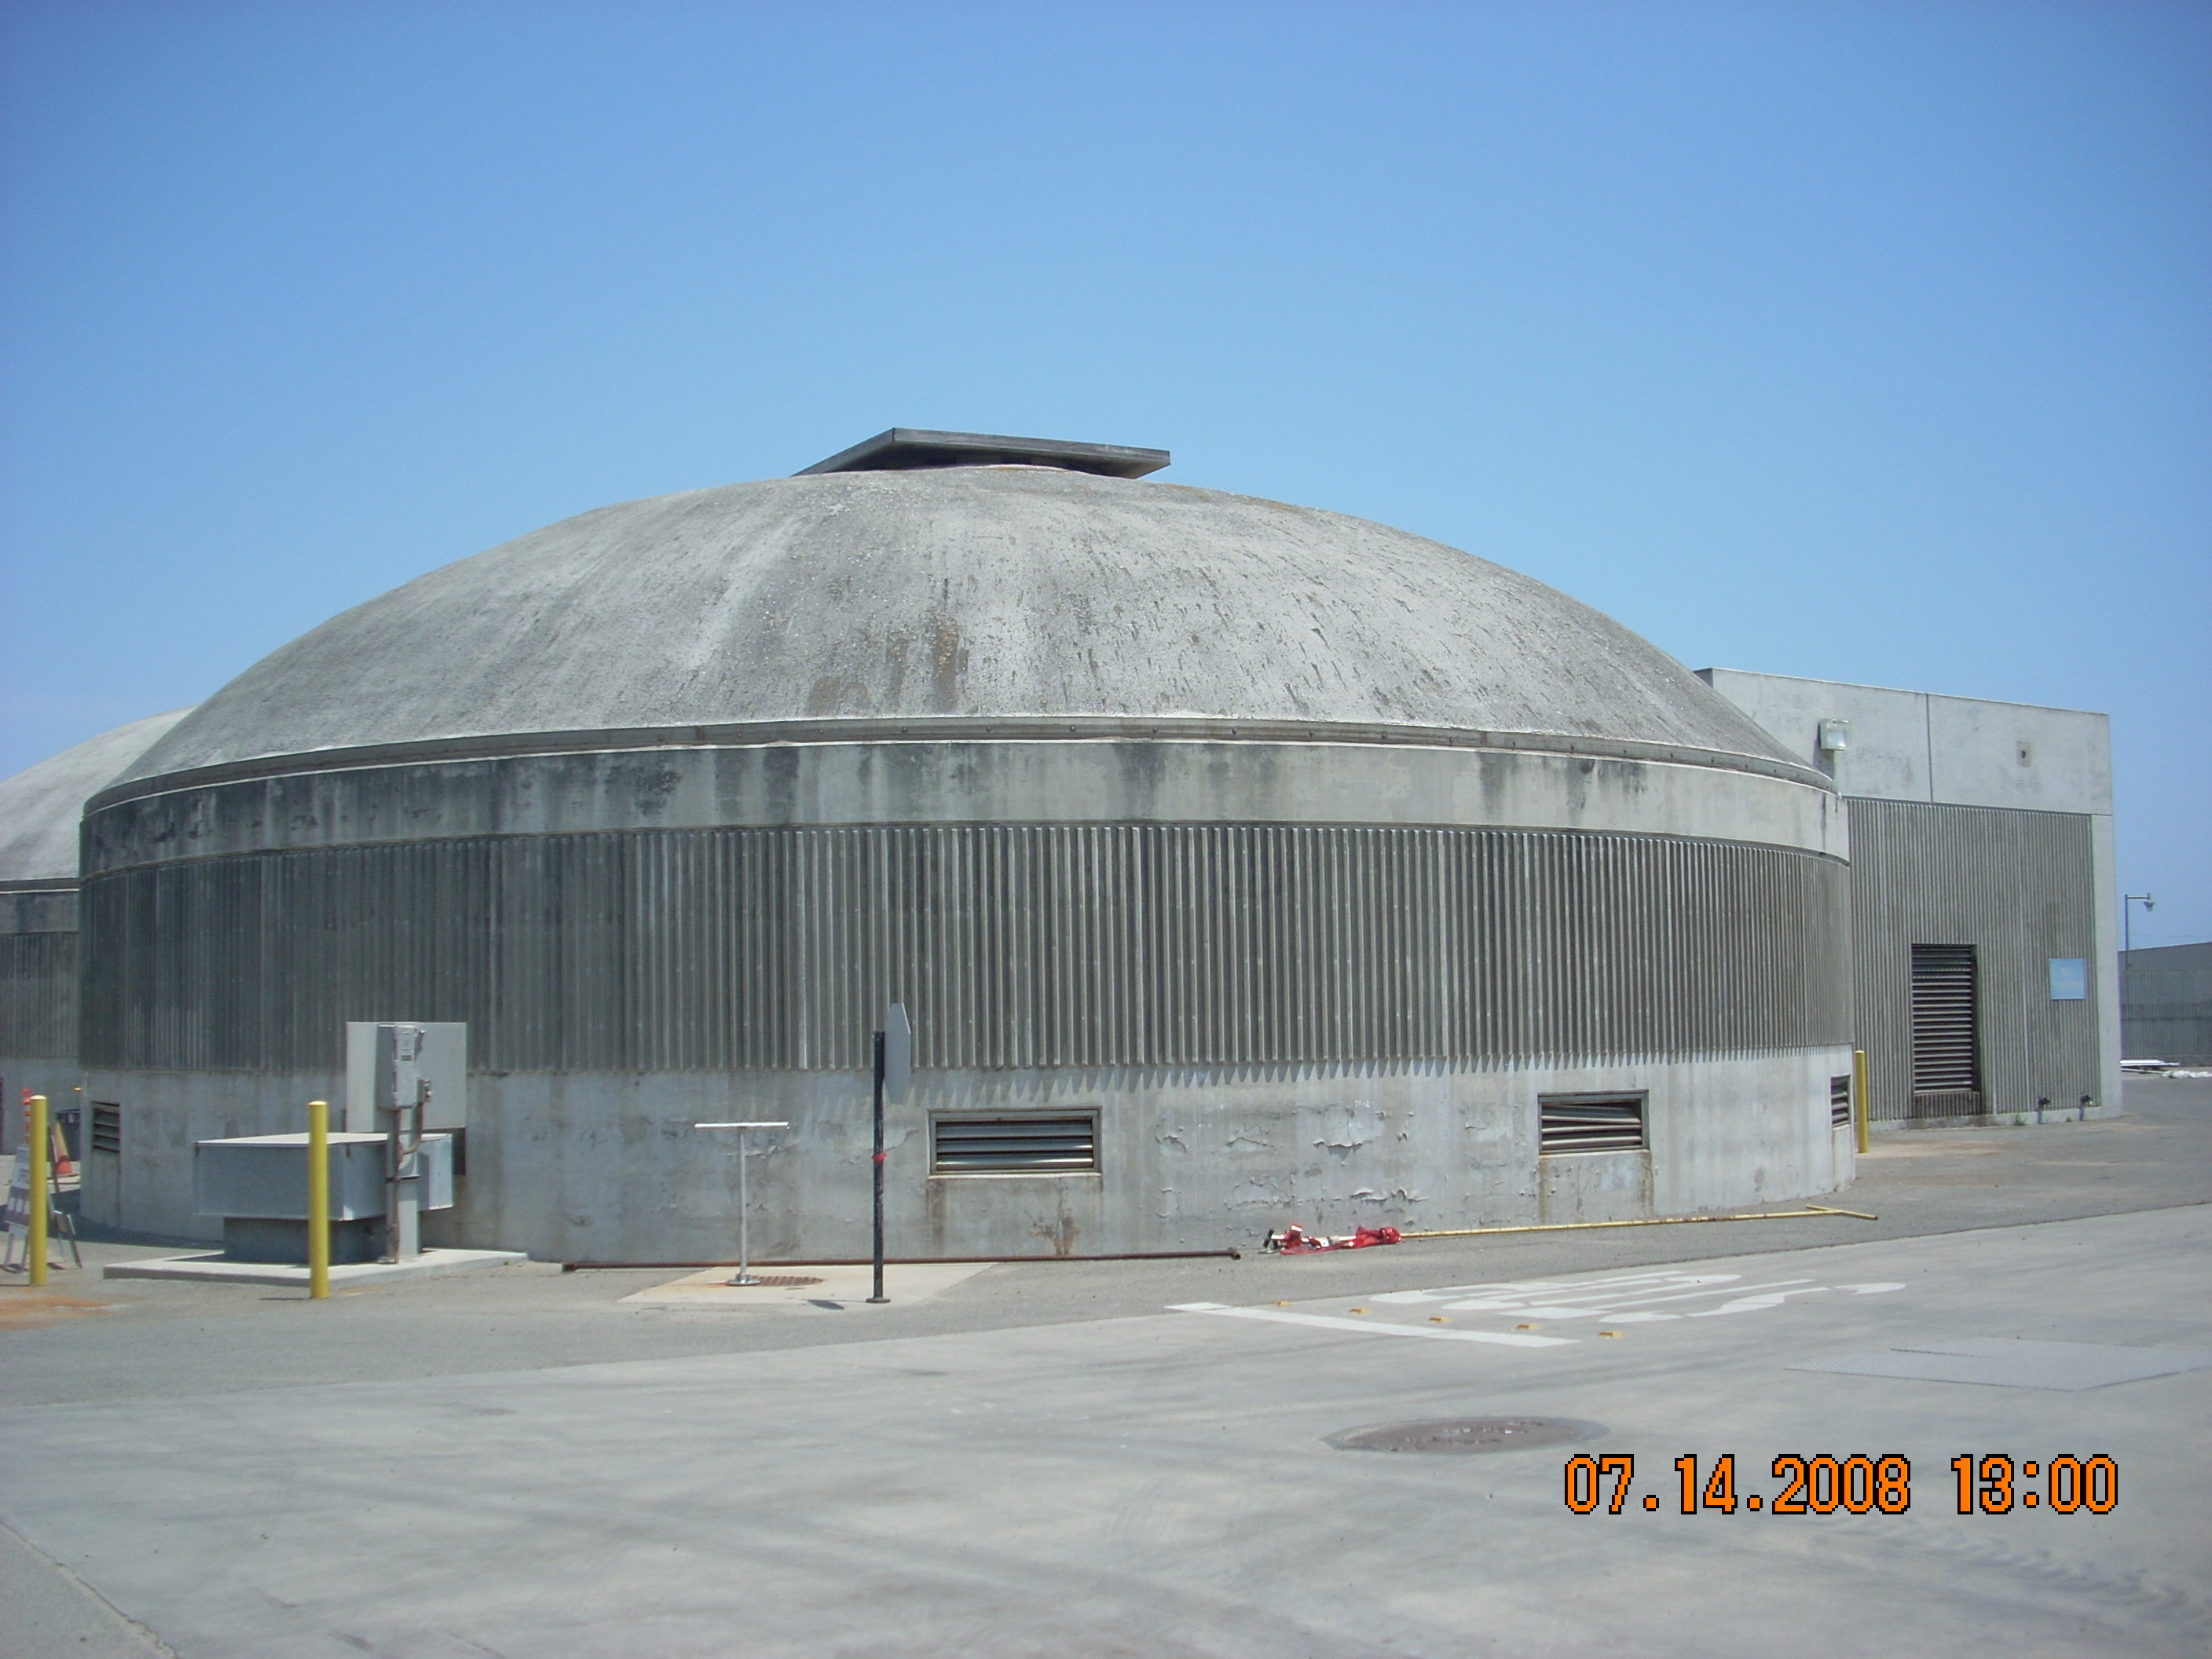
\includegraphics[scale=0.3]{DAFTOutside}\\
\vspace{1cm}
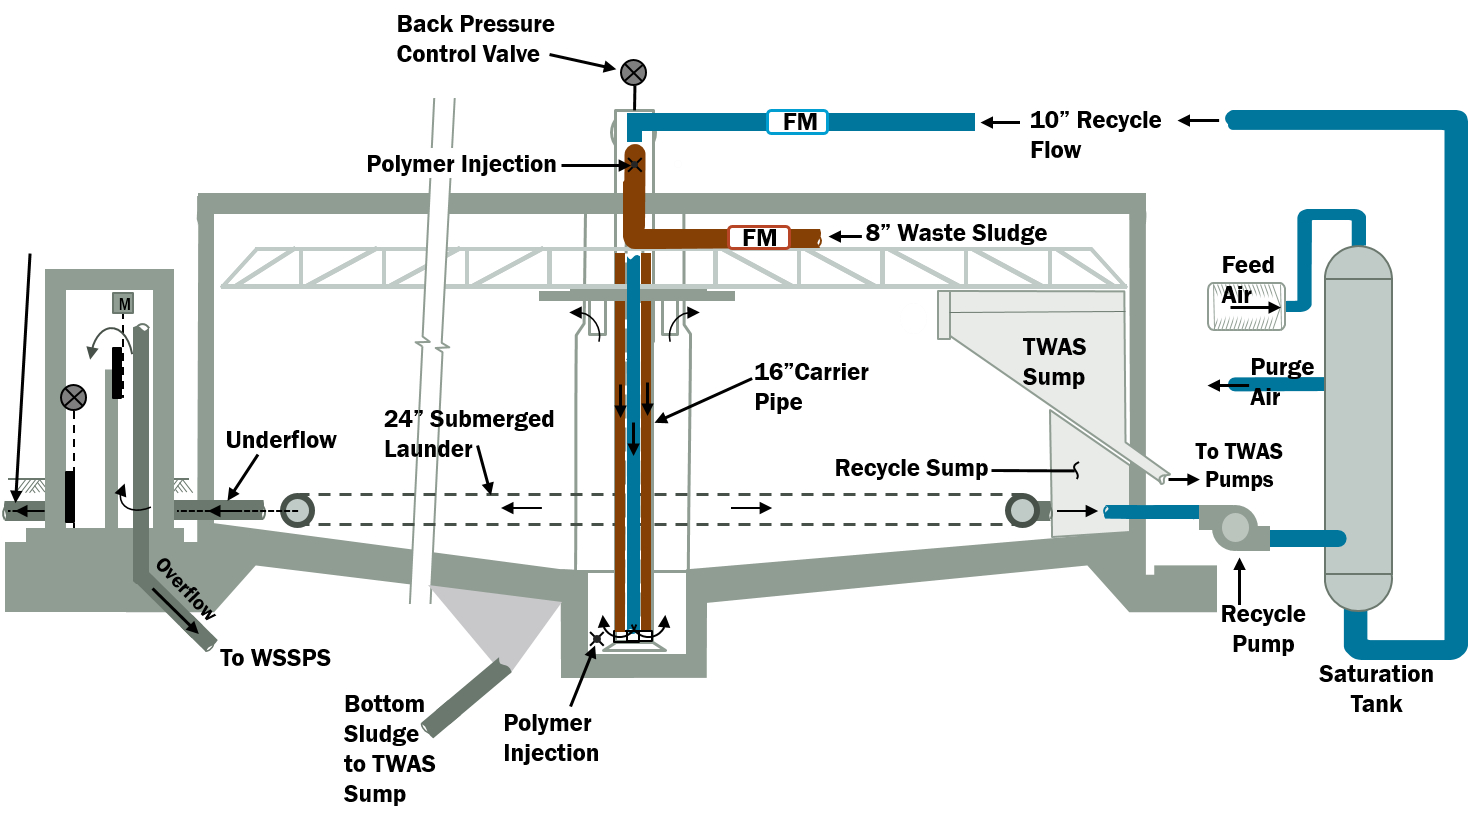
\includegraphics[scale=0.4]{DAFT}

\end{center}

\subsection{Principles of DAFT operations}\index{Principles of DAFT operations}

\begin{itemize}
\item WAS is conditioned with cationic polymer and introduced into the DAFT.  DAFTs typically operate at a solids loading rate of 1-2 lbs TSS/hr-ft$^2$.  Polymer feed ranges from 5-15 lbs of polymer/ton of the WAS (feed) solids.
\item Recycled water from the DAFT is pressurized with air in the saturation tank and mixed with polymer treated WAS as it is released at the bottom of the DAFT using the Back Pressure Control Valve.  
\item The dissolved air from the pressurized water is released as minute air bubbles rises upwards carrying with it the polymer flocculated sludge to the surface.  Adequate quantity of air is required to float the WAS solids.  Air:Solids ratio is one of the key operating and control parameter.  Typical air:solids ratios in a DAFT are between 0.03 - 0.05 lb air per lb TS. PS: Density of air used for air:solids ratio calculations - 0.075 lb air/ft$^3$ air - this value is given as part of the problem. 
\item The thickened solids floating on the top are scrapped off the surface of the DAFT by flights into the TWAS sump from where it is pumped to the digesters. The subnatant - water below the solids, part of it is used for the air pressurization in the saturation tank and the remaining is the underflow, which is returned back to the influent flow.
\item The flight speed is critical to the DAFT performance.  Fast flight speed would limit the thickness and density of the sludge blanket while slower flight speed would result in the thickened solids layer getting more dense and thick.  Excessively thick solids layer could result in the solids escaping through the underflow.  

\end{itemize}

\subsection{Elements of a DAFT}\index{Elements of a DAFT}

\begin{itemize}
\item pressurization or saturation tank 
\item thickened sludge skimmer with drive assembly
\item polymer dosing and injection system
\item thickened sludge pump
\item back pressure control valve
\item underflow removal
\item recycled flow system
\end{itemize}

\subsection{DAFT operational parameters}\index{DAFT operational parameters}

\begin{itemize}
\item saturation pressure
\item solids loading rate (lbs TSS/hr-$ft^2$)
\item hydraulic loading rate (GPD/$ft^2$/day)
\item feed solids concentration
\item detention period
\item air-to-solids ratio (lb air: lb solids)
\item type and quality of sludge
\item flight speed
\item solids and hydraulic loading rates, and
\item quantity and characteristics of the polymer used (lbs polymer/dry ton solids)
\end{itemize}


\newpage
\section*{Chapter Assessment}
\begin{tcolorbox}[breakable, enhanced,
colframe=blue!25,
colback=blue!10,
coltitle=blue!20!black,  
title= Chapter Assessment]

\begin{enumerate}


\item  In a gravity thickener the depth of the sludge is kept minimal (<six inches) to avoid solids going over the effluent weir \\

a. True \\
b. False \\

\item  Sludge thickening is primarily conducted to reduce costs associated with biosolids hauling\\


a. True \\
b. False \\


\item  Gravity thickener is commonly used for sludge dewatering \\

a. True \\
b. False \\

\item  Sludge thickening is primarily conducted to reduce costs associated with biosolids hauling \\

a. True \\
b. False \\
\item A DAF thickener has effluent solids of 55 mg/L and float solids of 2.0\%. Solids loading and polymer dosing is in the normal range. This data likely indicates: \\

a. This unit is operating normally \\
b. Too low air to solids ratio \\
c. Float blanket too thick \\
d. Flight speed too fast \\
e. Flight speed too slow \\

\item  An air flotation thickener will produce a thin float if: \\

a. Flight speed too high and skimmer wiper not adjusted properly \\
b. Excessive air/solids ratio and polymer dosages too low \\
c. High dissolved oxygen and flight speed too low \\
d. Polymer dosages too high and unit overloaded \\

\item  An increase in the pool depth of a scroll-type centrifuge: \\

a. would not affect the moisture content of the cake. \\
b. would produce a drier cake \\
c. would produce a wetter cake, but produce a greater solids recovery. \\
d. would not affect either solids recovery, nor cake moisture content. \\
e. would require an increase in the cationic polymer dosage. \\

\item  A sludge thickened from 1\% to 4\% solids will be reduced in volume by how much? \\

a. no more than 4\% of original volume \\
b. approximately 17\% of original volume \\
c. approximately 25\% of original volume \\
d. more information is needed \\

\item  Gravity thickeners, compared to DAFs, are best suited to: \\

a. Thickening primary sludge. \\
b. Thickening waste activated sludge. \\
c. Controlling sulfide odors. \\
d. Removing filamentous bacteria. \\
e. Provide highest concentration sludge. \\

\item  Which of the following is not the main reason for thickening sludge \\

a. Improved digester performance due to a lower volume of sludge \\
b. Cost savings in the construction of new digestion facilities \\
c. Reduction in anaerobic digestion heating requirements since less water has to be heated \\
d. Reduce costs of biosolids hauling \\
\end{enumerate}
\end{tcolorbox}